% Chapter Template

\chapter{VIRTUOSO INSTALLATION AND MANIPULATION} % Main chapter title

\label{Chapter8} % Change X to a consecutive number; for referencing this chapter elsewhere, use \ref{ChapterX}

\lhead{Chapter 8. \emph{VIRTUOSO INSTALLATION AND MANIPULATION}} % Change X to a consecutive number; this is for the header on each page - perhaps a shortened title


Although forensic memory analysis community has developed plenty of utilities which could be leveraged for VM introspection, 
VMI applications based on these utilities such as volatility plugin, are still not able to be applied conveniently in for example 
operator provided cloud environment. The reason is obvious: the approach strongly depends on the stability of target VM kernel. 
Once update or patch is applied to monitored guest’s kernel, these VMI applications may need to be adapted. 
To remedy this mentioned problem, some VMI applications depending on reutilizing binary code, such as VIRTUOSO, are presented. 
As far as I know, VIRTUOSO is the unique open source tool in this domain. Therefore, we will introduce in this section the installation 
and manipulation of VIRTUOSO.


%----------------------------------------------------------------------------------------
%	SECTION 1
%----------------------------------------------------------------------------------------

\section{Installation of VIRTUOSO}

A rather detailed and helpful how-to wiki about installation of VIRTUOSO is available in the link: 
https://code.google.com/p/virtuoso/wiki/Installation. Since that this wiki has not seen any update since 2012, 
we were still stuck by some unexpected problems.  As a meaningful complement to the initial how-to wiki, this tutorial aims to record 
all crossed problems and its solution in the road of VIRTUOSO exploration.

To install VIRTUOSO, 64-bit Linux system (Debian/Ubuntu preferred) and Python 2.6 or later are required. Its source code is 
http://code.google.com/p/virtuoso/downloads/list. After obtaining the VIRTUOSO source code, it consists of two steps to install VIRTUOSO:
install all dependencies for VIRTUOSO (gcc 3.4, QEMU 0.9.1, libdasm), compile and install iFerret.

%-----------------------------------
%	SUBSECTION 1
%-----------------------------------
\subsection{Problem 1: No SDL support for installation of QEMU 0.9.1}
The first obstacle encountered appears during the installation of QEMU 0.9.1, which is shown in Figure \ref{fig:No SDL support for installation of QEMU 0.9.1}.

\begin{figure}[htbp]
	\centering
		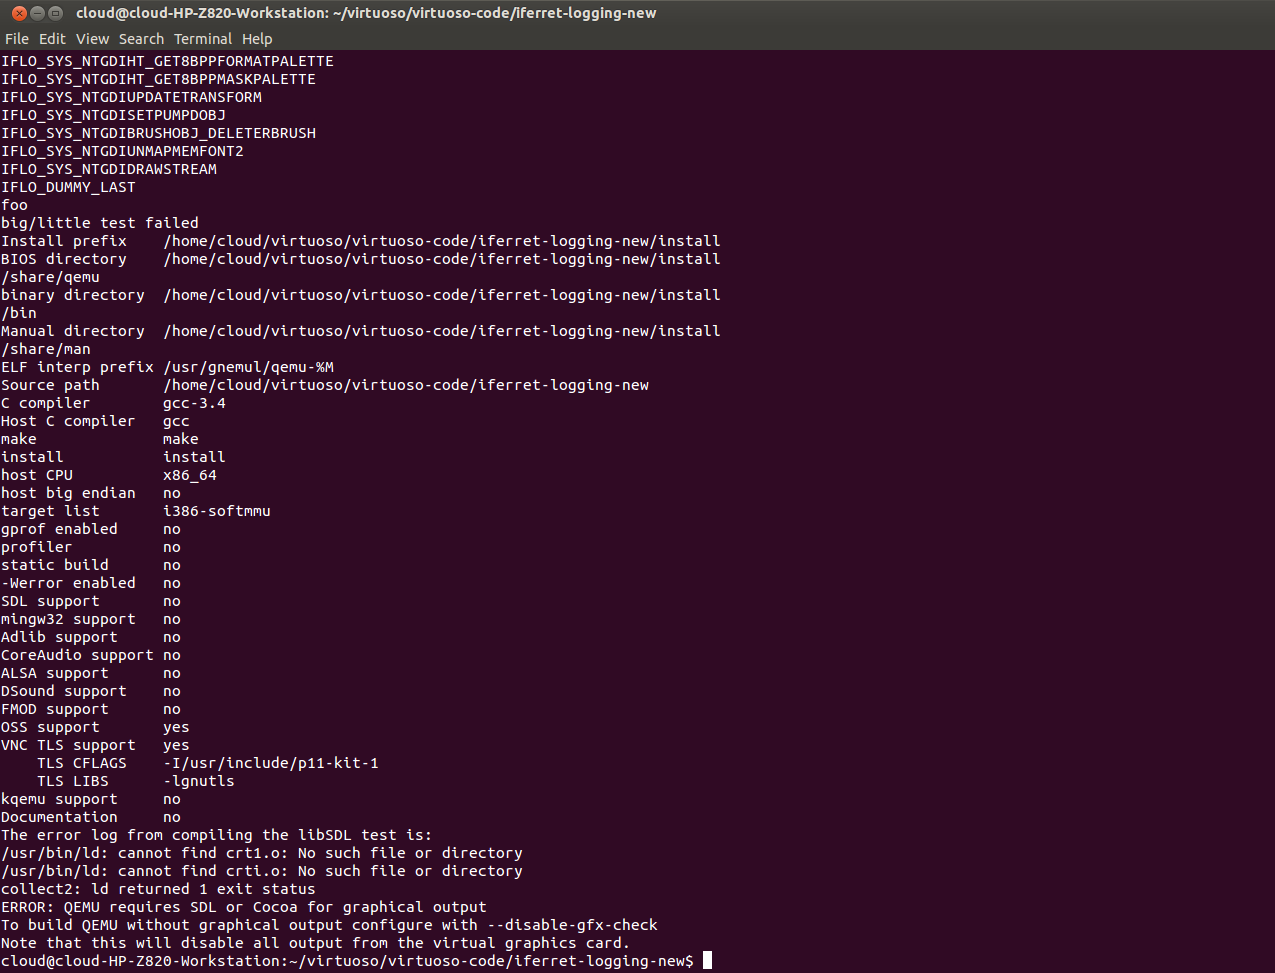
\includegraphics[width=14cm, height= 9cm ]{Figures/Figure32.png}
	\caption[No SDL support for installation of QEMU 0.9.1]{No SDL support for installation of QEMU 0.9.1}
	\label{fig:No SDL support for installation of QEMU 0.9.1}
\end{figure}

The cause of this error lies in that system could not find graphical output support for QEMU 0.9.1(notice that SDL support check's 
result is no.). After some searching online, I found a solution to this problem: It should issue the following command in the terminal a prior to installing iFerret component of VIRTUSO:
\shellcmd{export LIBRARY\_PATH=/usr/lib/x86\_64-linux-gnu}
With this export command, system is able to find the path to libSDL library required by QEMU 0.9.1.

%-----------------------------------
%	SUBSECTION 2
%-----------------------------------

\subsection{Problem 2: iFerret compile error}
The error is occurred when we change into the 'iferret-logging-new' directory and issue 'make install' command, as shown in Figure \ref{fig:iFerret compile error}.

\begin{figure}[htbp]
	\centering
		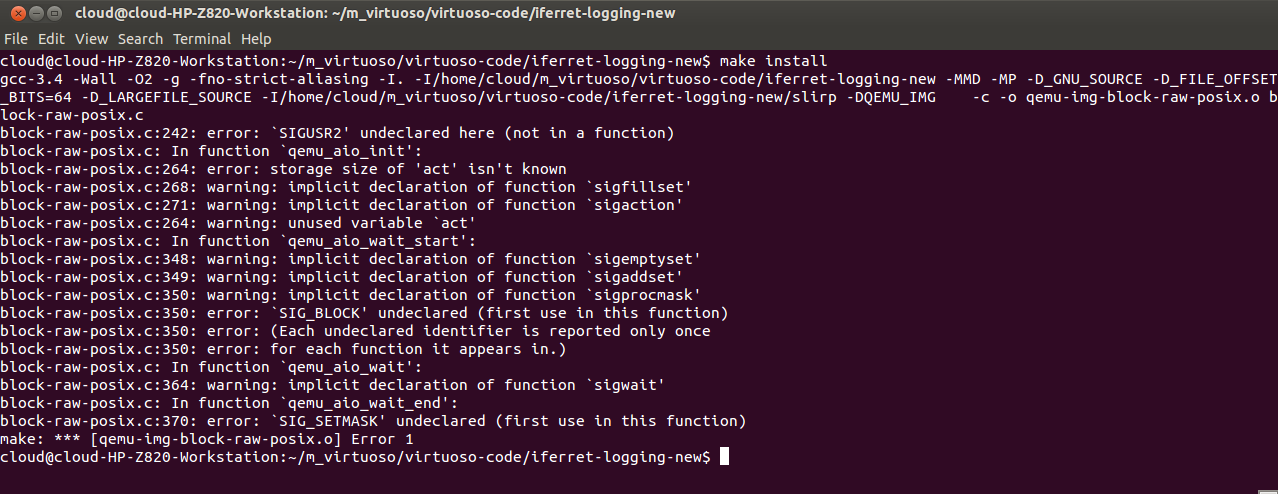
\includegraphics[width=14cm, height= 9cm ]{Figures/Figure33.png}
	\caption[iFerret compile error]{iFerret compile error}
	\label{fig:iFerret compile error}
\end{figure}

Obviously, from above figure, we could infer that there exist some bugs in source file ‘block-raw-posix.c’. After some investigation, 
this is caused by a macro definition syntax. Look at the block of code shown in Figure \ref{} which causes the above error:

\begin{figure}[htbp]
	\centering
		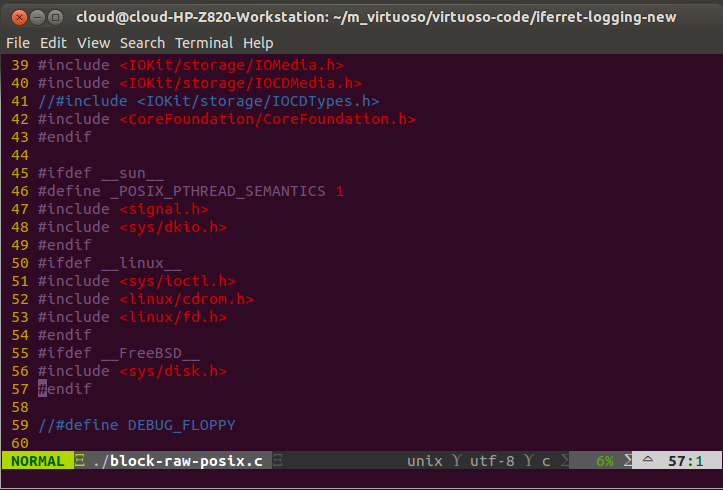
\includegraphics[width=14cm, height= 9cm ]{Figures/Figure34.png}
	\caption[Bloc of code causing compile error]{Bloc of code causing compile error}
	\label{fig:Bloc of code causing compile error}
\end{figure}

C header file ‘signal.h’ is included under some conditions. To solve this problem, it simply needs to  add one line instruction at the 
beginning of this file: \#include <signal.h>. Repeat 'make install' command, normally, no errors will appear and the installation process 
should be finished with success. Now you could give a try to VIRTUOSO following another wiki in its official site.

\subsection{Problem 3: The abort of execution of example VM image}
Issuing the command line:
\shellcmd{install/bin/qemu -m 256 -hda haiku-r1alpha2-anyboot.qcow2 -usbdevice tablet\\ -loadvm introprog -monitor stdio -k en-us -iferret\_log walkthrough}
However, new error has occurred:

\begin{figure}[htbp]
	\centering
		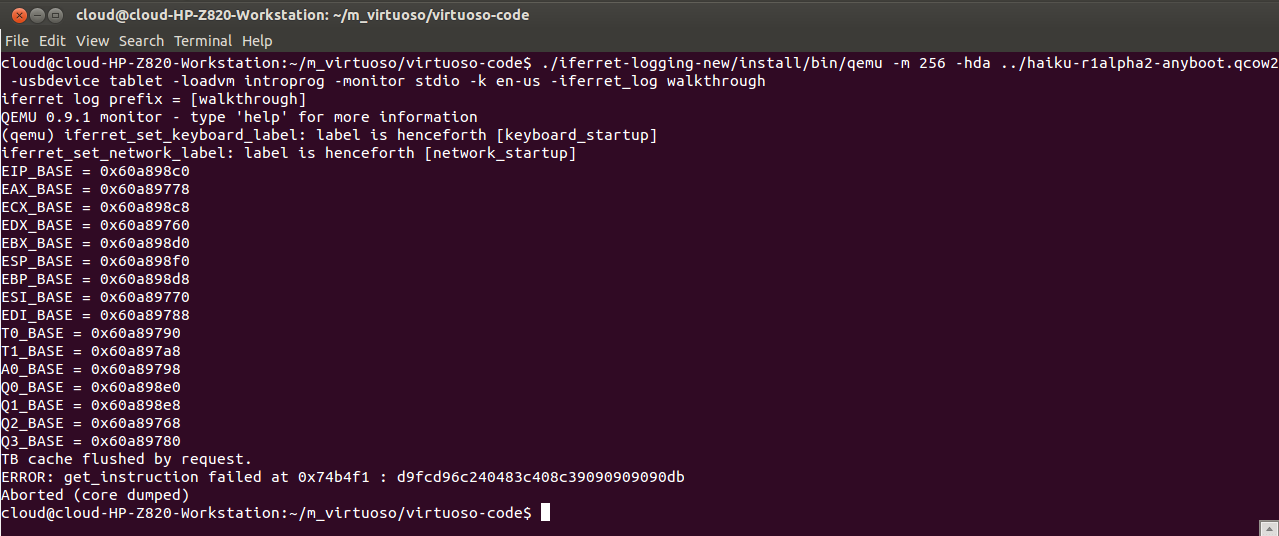
\includegraphics[width=14cm, height= 9cm ]{Figures/Figure35.png}
	\caption[Abort of execution of example VM image]{Abort of execution of example VM image}
	\label{fig:Abort of execution of example VM image}
\end{figure}

This error is not evident as others obstacles we encountered before and nothing could be found online. After one week’s effort, 
I finally got some clues about this problem to read another wiki 'limitation' at https://code.google.com/p/virtuoso/wiki/Limitations,
This is caused by the fact that:

\textcolor{blue}{
  "Virtuoso makes use of libdasm to disassemble instructions (see iferret-logging-new/target-i386/translate.c for details). 
  Libdasm is missing support for some instructions, and this will cause tracing to stop and QEMU to shut down. The disassembly Virtuoso does 
  is mainly for debugging, and so these lines can be commented out if they cause trouble. I would like to switch to a more reliable disassembler 
  in the future, however."
}

Therefore, the answer to the problem is: libdasm encountered some unknown instructions in Ubuntu14.04 and forces VIRTUOSO to abort. 
To solve this, we need to identify and comment related block of code in file 'translate.c' and recompile all. Concretely, comment line 
from 3281 to 3335 in file ‘iferret-logging-new/target-i386/translator.c’ and recompile install all. 

Until now, we could take a ride with VIRTUOSO. Change into directory ‘iferret-logging-new’ and issue the following command line into a 
terminal:
\shellcmd{install/bin/qemu -m 256 -hda haiku-r1alpha2-anyboot.qcow2 -usbdevice tablet\\ -loadvm introprog -monitor stdio -k en-us -iferret\_log walkthrough}
Some explanation about above command: To prove that VIRTUOSO is OS-angostic VMI technology, we use a Haiku OS-based virtual machine image provided.
by author. This virtual machine comes with a snapshot named "introprog" that has a few training programs already loaded and compiled. 
For example, we could run a training program named "enumprocs" to get the PID list of currently running process in guest virtual machine.
The execution result is shown in Figure \ref{fig:Run Training program in trusted VM}.
\begin{figure}[htbp]
	\centering
		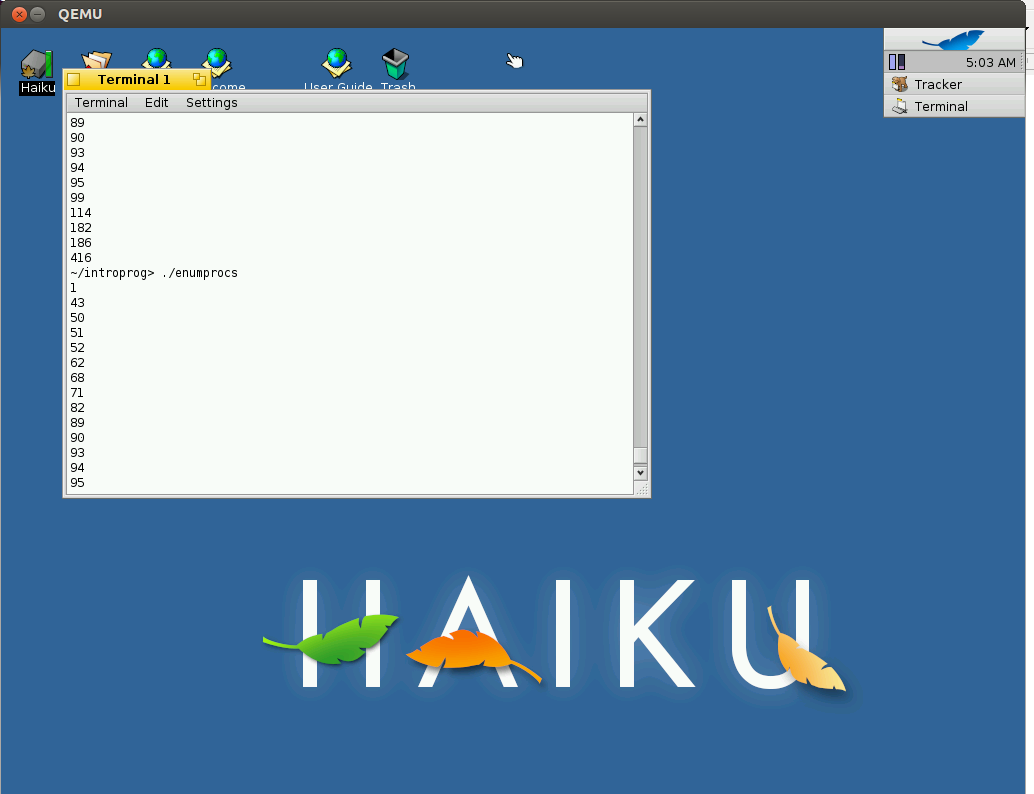
\includegraphics[width=14cm, height= 9cm ]{Figures/Figure36.png}
	\caption[Run Training program in trusted VM]{Run Training program in trusted VM}
	\label{fig:Run Training program in trusted VM}
\end{figure}

Notice that, after several times of invocation of small programs such as 'enumprocs', we observe that some execution traces files are 
generated.  Generated output file will be placed in directory where VIRTUOSO is called. (In this case, it is directory 'iferret-logging-new')

\subsection{Problem 4: IPython runtime exception when generating inspection code with VIRTUOSO}
Given that, component ‘iFerret’ of VIRTUOSO has obtained execution traces of training program, it is time to analysis trace file and 
produces the Volatility plugin. To achieve this, go to the dynslicer directory and run:
\shellcmd{./newslicer.py -o haiku ../iferrret-logging-new/walkthrough.0-17864}
Unfortunately, there comes a new error:

\begin{figure}[htbp]
	\centering
		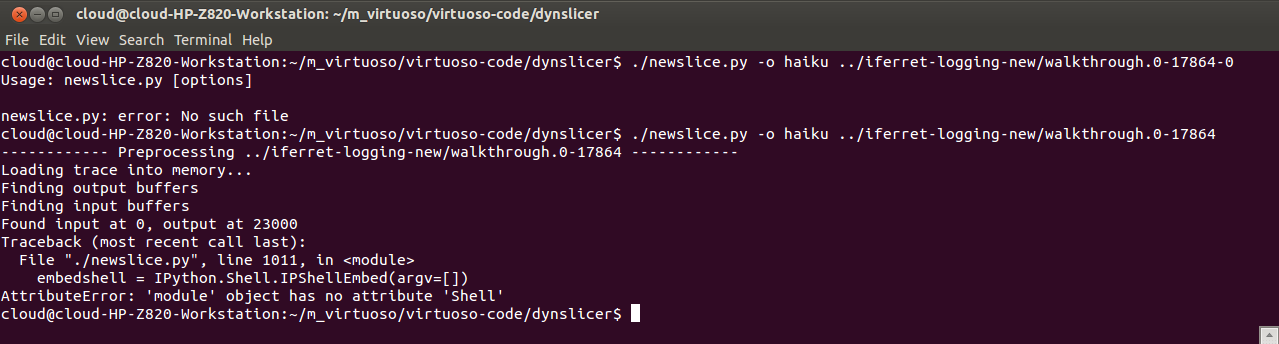
\includegraphics[width=14cm, height= 9cm ]{Figures/Figure37.png}
	\caption[IPython run exception]{IPython run exception}
	\label{fig:IPython run exception}
\end{figure}

Definitely, this is related to the IPython version installed in our workstation. A possible solution to this problem is:
\shellcmd{sudo pip uninstall ipython\\\# sudo pip --proxy=http://proxy.rd.francetelecom.fr:8080 install ipython==0.10}
Then re-execute above invocation, and output is shown in Figure \ref{fig:VIRTUOSO introspection tool generation}.
\begin{figure}[htbp]
	\centering
		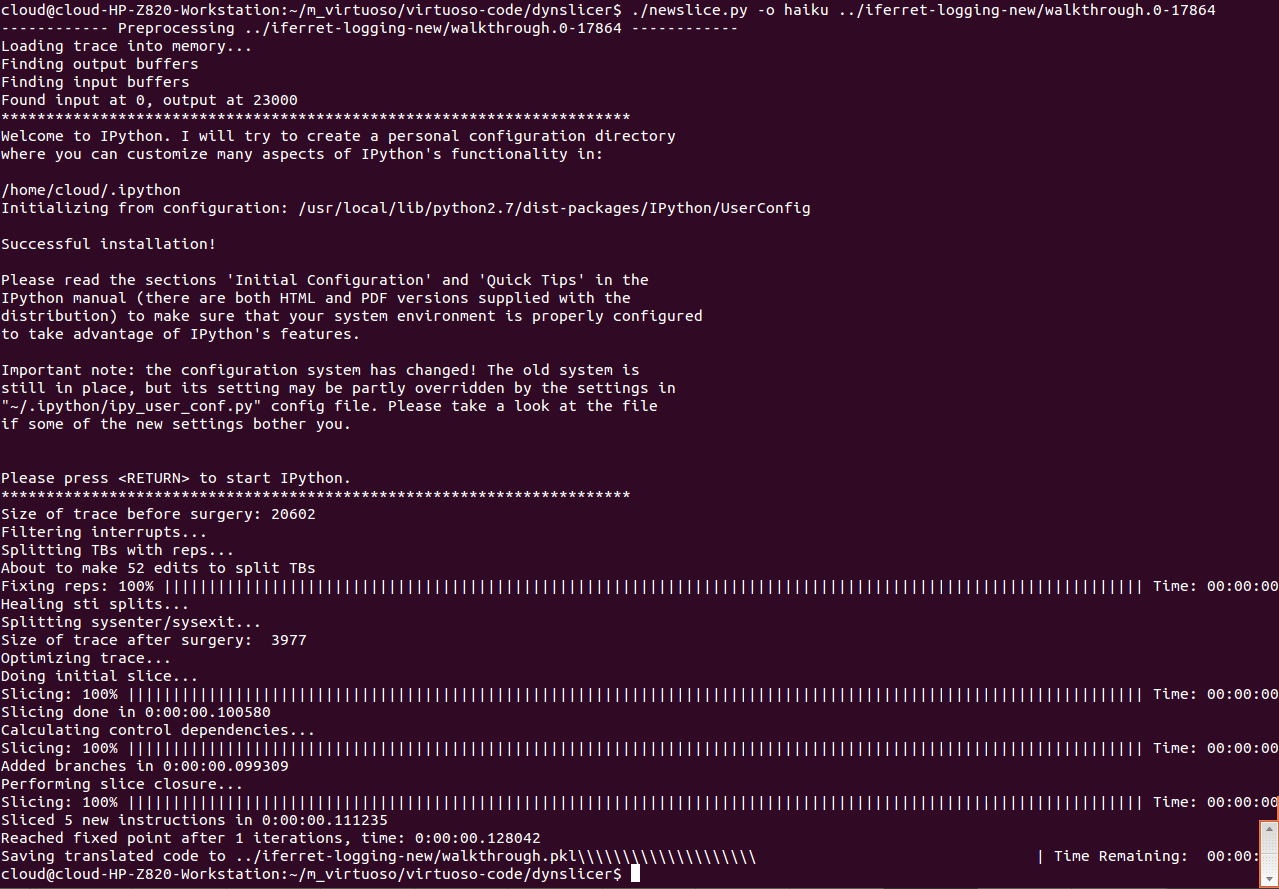
\includegraphics[width=14cm, height= 9cm ]{Figures/Figure38.png}
	\caption[VIRTUOSO introspection tool generation]{VIRTUOSO introspection tool generation}
	\label{fig:VIRTUOSO introspection tool generation}
\end{figure}
When Volatility plugin is well generated, we could profit to realize introspection job at the level of hypervisor and get mostly the 
same view as inside the monitored VM. To do this, change into volatility-1.3-Beta directory and tape the following command:
\shellcmd{./volatility newmicrodo -f ../iferret-logging-new/walkthrough.0.mem \textbackslash\\ -e ../iferret-logging-new/walkthrough.0.env\textbackslash\\ -m ../iferret-logging-new/walkthrough.pkl\textbackslash\\ -n ' [ mem.alloc(1024) ] ' -i 'def f(x): print unpack("<\%dI" \% (len(x)/4),x)'}

\begin{figure}[htbp]
	\centering
		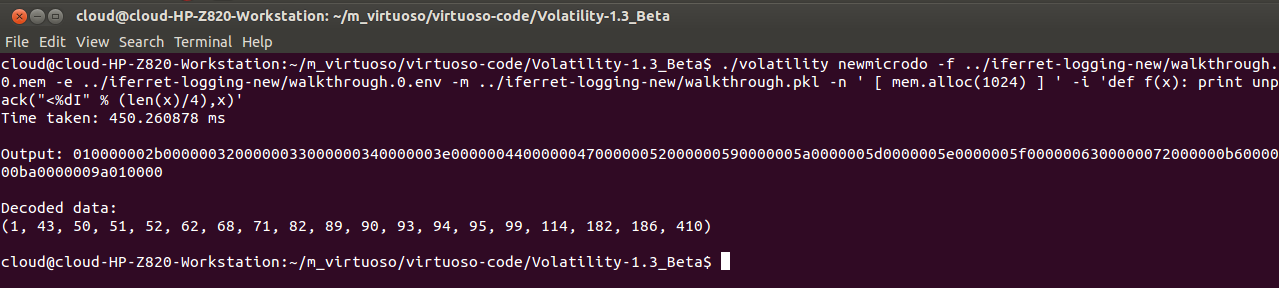
\includegraphics[width=14cm, height= 7cm ]{Figures/Figure39.png}
	\caption[VIRTUOSO introspection tool execution result]{VIRTUOSO introspection tool execution result}
	\label{fig:VIRTUOSO introspection tool execution result}
\end{figure}

\section{Assessment of VIRTUOSO}
Traditionally, the principal philosophy was to imitate the existing inspecting utility (ps, netstat command in Linux for example.) 
and rewrite the code from scratch with an intimate knowledge of OS kernel. This approach is rather intuitive but at the same time 
presents some obvious disadvantages:

\begin{itemize}
    \item Prone to import new security when writing new introspection utilities
    \item Has to adapt each time target OS kernel has some updates
    \item Need much human effort
 \end{itemize}
The greatest significance of VIRTUOSO lies in that it breaks away from conventions and leverages the reutilization of
binary code. Exception the training stage, VIRTUOSO is capable of automatically generating introspection tool with 
obtained execution traces without target OS kernel knowledge.

However, the limitation of VIRTUOSO is also evident: first, it is not still completely automatic in generating introspection
tool. VIRTUOSO still needs an expert to write the training programs to get system API execution traces in which we are
interested. This expert is supposed to have an intimate knowledge about target system API, for example, which API is used 
to get the list of running processes in Haiku operating system. When writing training program, he should also assure that
there is no process switch (context switch) during training program execution. In one word, it is a little difficult to 
write training program. Second, the range of introspection tools generated by VIRTUOSO depends on the target OS API, 
due to the fact that VIRTUOSO just simply reutilizes binary code s associated with system API. Third, VIRTUOSO is not
able to extract device I/O code or instruction, VIRTUOSO is therefore not capable of generating network-side introspection
tools. All above constraints hinder the application of VIRTUOSO in industry, but its philosophy inspired other interesting 
introspection tool, such as VMST.




